
\section{Desarrollo de los modulos}
En este capítulo se destacaron las partes más importantes del desarrollo de los módulos, enfocándonos en los aspectos clave que contribuyeron a su implementación exitosa y al cumplimiento de los objetivos propuestos.
Para el desarrollo de los módulos, es importante destacar que, al igual que la plataforma que los contiene, se utilizó React, una biblioteca de código abierto basada en JavaScript, la cual facilita la creación de interfaces de usuario dinámicas y eficientes. A continuación, se detallan los elementos utilizados en la creación de los dos módulos de fitness: uno enfocado en ayudar a mantener una buena postura de la espalda y otro en la prevención del síndrome del túnel carpiano. También se describe el módulo de mindset, diseñado para fortalecer habilidades como la interpretación de patrones, el autocontrol, la adaptabilidad, entre otras. Todo lo desarrollado se encuentra disponible en https://github.com/azcaratejuan/soft-skills-plataform \subsection{Modulo fitness}
\subsubsection{Modulo fitness: Ejercicios para el tunel carpiano}
Para el desarrollo de la primera gamificacion especificamente para prevenir el síndrome del túnel carpiano, se decidió utilizar tecnologías capaces de reconocer las poses de las manos. En este caso, se empleó TensorFlow de Google, específicamente el modelo Handpose, el cual identifica 21 puntos clave en la mano, incluyendo todas las articulaciones de los dedos y las puntas de los mismos. Estos puntos se utilizan para calcular poses específicas mediante el uso de inteligencia artificial.
\\
Como consecuencia, se diseñó un juego que aprovecha diferentes posiciones de las manos para prevenir el síndrome del túnel carpiano, siguiendo las recomendaciones descritas en el documento "Síndrome del Túnel Carpiano: Protocolo de Tratamiento Conservador"\cite{14_1}. Las posiciones de la mano se usan en el juego para realizar acciones como subir, bajar o esquivar obstáculos, tal como se demuestra en la siguiente imagen:
\begin{figure}[H]
  \centering
  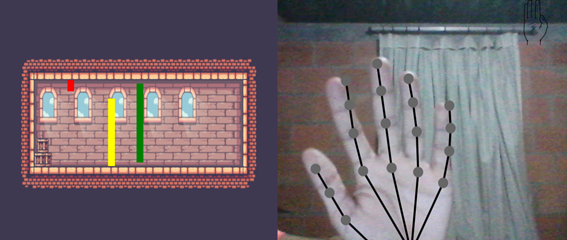
\includegraphics[width=0.6\linewidth]{Imagenes/Fitness1.png}
  \caption{Módulo fitness, imagen de muestra de gamificación sobre el túnel carpiano. Elaboración propia}
  \label{fig:imagen1fitness}
\end{figure}


Posteriormente, se añadieron otros elementos gamificados, como un contador que mide el tiempo que el jugador ha resistido, con el objetivo de incentivar al usuario a alcanzar el mayor puntaje posible. Estos elementos añaden dinamismo y motivación,Ademas se agregaron los botones para iniciar/pausar  y uno para reiniciar el juego como se ilustra en la siguiente imagen:

\begin{figure}[H]
  \centering
  
\includegraphics[width=0.6\linewidth]{Imagenes/Fitness2.png}
  \caption{Módulo fitness, imagen de muestra sobre botones y elemento puntuación de gamificación sobre el túnel carpiano. Elaboración propia}
  \label{fig:imagen2fitness}
\end{figure}

Finalmente, se añadió una imagen inicial con instrucciones para que el jugador comprendiera tanto los botones como las posiciones que deberá usar durante el juego:
\begin{figure}[H]
  \centering
  \includegraphics[width=0.5\linewidth]{Imagenes/tutorial-muñeca.png}
  \caption{Módulo fitness, imagen de las instrucciones sobre gamificación del túnel carpiano. Elaboración propia}
  \label{fig:imagen3fitness}
\end{figure}



\subsubsection{Modulo fitness: Ejercicios para la corrección de la mala postura de la espalda}
Para el desarrollo de la segunda parte del módulo de fitness, se decidió utilizar tecnologías capaces de detectar poses en este caso también de Google llamada Media-Pipe en su apartado hand landmarks. El cual identifica la posición de las manos en pantalla mediante inteligencia artificial.
\\
A partir de esta tecnología, se decidió desarrollar un juego enfocado en estiramientos para la espalda. Aprovechando la detección de la posición de las manos, el juego está diseñado para promover estiramientos básicos, incentivando al usuario a cambiar la posición de las manos de manera constante. Se emplean varias posiciones predefinidas, que guían al usuario a realizar los movimientos correctos para mejorar su postura y prevenir dolores asociados a la mala alineación de la espalda. A continuación, se muestran las posiciones utilizadas:
\begin{figure}[H]
  \centering
  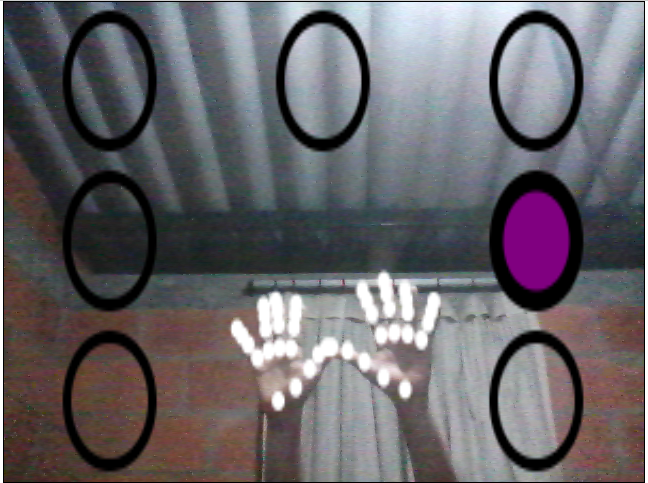
\includegraphics[width=0.6\linewidth]{Imagenes/Fitness3.png}
  \caption{Módulo fitness, imagen de muestra sobre gamificación para la corrección de mala postura en la espalda. Elaboración propia}
  \label{fig:imagen4fitness}
\end{figure}


Como resultado, se implementó un sistema en el que, al seleccionar una canción, se muestra una serie de movimientos que el usuario debe seguir, complementado con la reproducción de música para hacer la experiencia más agradable. Al igual que en el módulo anterior, se añadieron elementos gamificados, como un contador que mide la cantidad de movimientos correctos realizados por el usuario, incentivando así a alcanzar el mayor puntaje posible. Además, se incorporaron botones de iniciar y pausar para una mejor interacción, como se muestra en la siguiente imagen:


\begin{figure}[H]
  \centering
  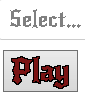
\includegraphics[width=0.1\linewidth]{Imagenes/Fitness4.png}
  \caption{Módulo fitness, imagen de muestra sobre botones de la gamificación para la corrección de mala postura en la espalda. Elaboración propia}
  \label{fig:imagen5fitness}
\end{figure}

\begin{figure}[H]
  \centering
  
\includegraphics[width=0.2\linewidth]{Imagenes/Fitness5.png}
  \caption{Módulo fitness, imagen de muestra sobre elemento puntuación sobre gamificación para la corrección de mala postura en la espalda. Elaboración propia}
  \label{fig:imagen6fitness}
\end{figure}

Finalmente, se añadió una imagen inicial con instrucciones para que el jugador comprendiera tanto los botones como las posiciones que deberá usar durante el juego:
\begin{figure}[H]
  \centering
  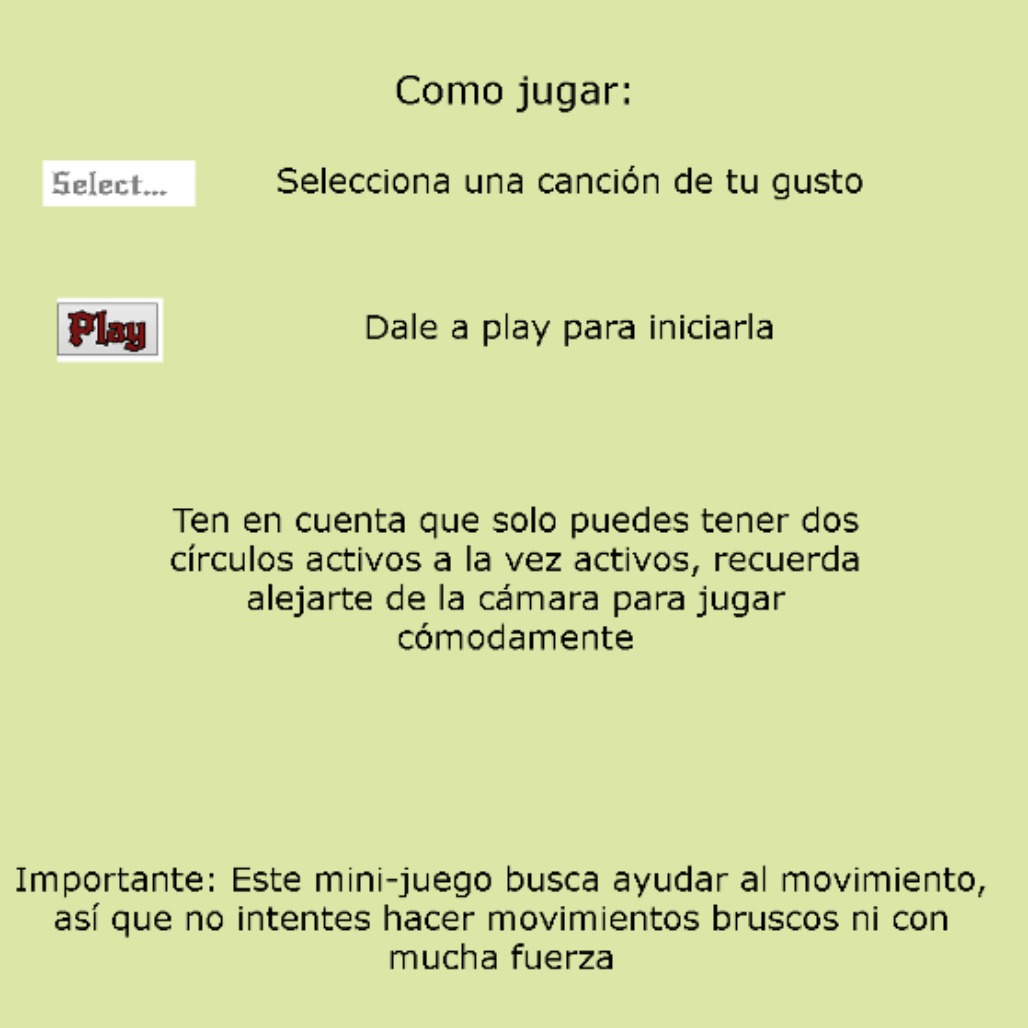
\includegraphics[width=0.5\linewidth]{Imagenes/tuto-espalda.png}
  \caption{Módulo fitness, imagen de tutorial sobre gamificación para la corrección de mala postura en la espalda. Elaboración propia}
  \label{fig:imagen7fitness}
\end{figure}

\subsection{Modulo mindset}
En el desarrollo del módulo de mindset, se decidió agrupar las subhabilidades seleccionadas en el capítulo anterior y utilizar el motor de videojuegos Godot, conocido por su capacidad para crear entornos 2D y 3D multiplataforma, libre y de código abierto. Para este caso de estudio, se optó por usar principalmente su funcionalidad en 2D, desarrollando una serie de niveles enfocados en fomentar habilidades como la capacidad analítica, la interpretación de patrones y la creatividad, entre otras previamente mencionadas. Estos niveles abarcan desde el uso de una balanza para decidir la posición de bloques hasta la interpretación de patrones para elegir el siguiente camino a seguir. A continuación, se presentan los diferentes niveles junto con un breve resumen de cada uno.
\subsubsection{Nivel 1}
El primer nivel se basa en una agrupación de flechas dentro de un laberinto sencillo. La idea es enseñar al jugador que puede interactuar con los objetos, fomentando así la exploración y la interacción en el entorno de juego.

\begin{figure}[H]
  \centering
  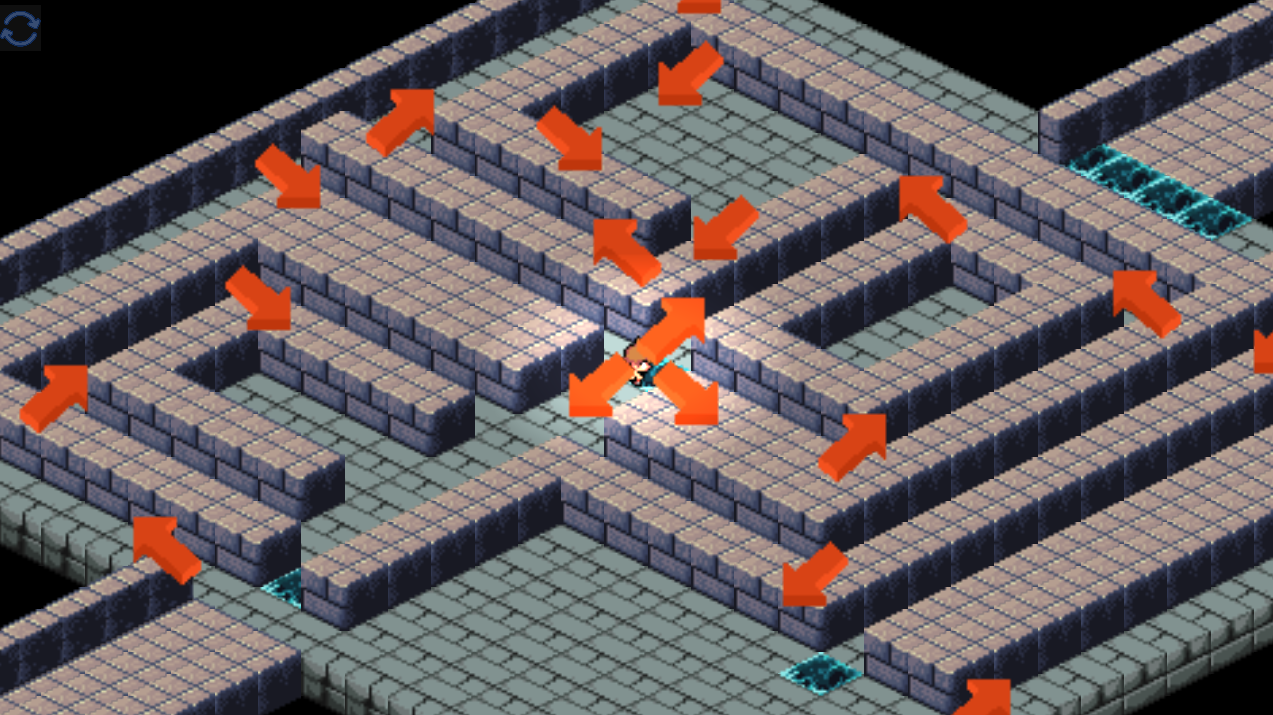
\includegraphics[width=0.7\linewidth]{Imagenes/Nivel1.png}
  \caption{Módulo mindset, imagen de referencia sobre gamificación para el módulo mindset, Nivel 1. Elaboración propia}
  \label{fig:imagen1mindset}
\end{figure}


\subsubsection{Nivel 2}

El segundo nivel se basa en una balanza con la cual el jugador debe interactuar para comparar el peso de dos objetos y ordenarlos según su peso. Este nivel busca fomentar el razonamiento lógico del jugador.

\begin{figure}[H]
  \centering
  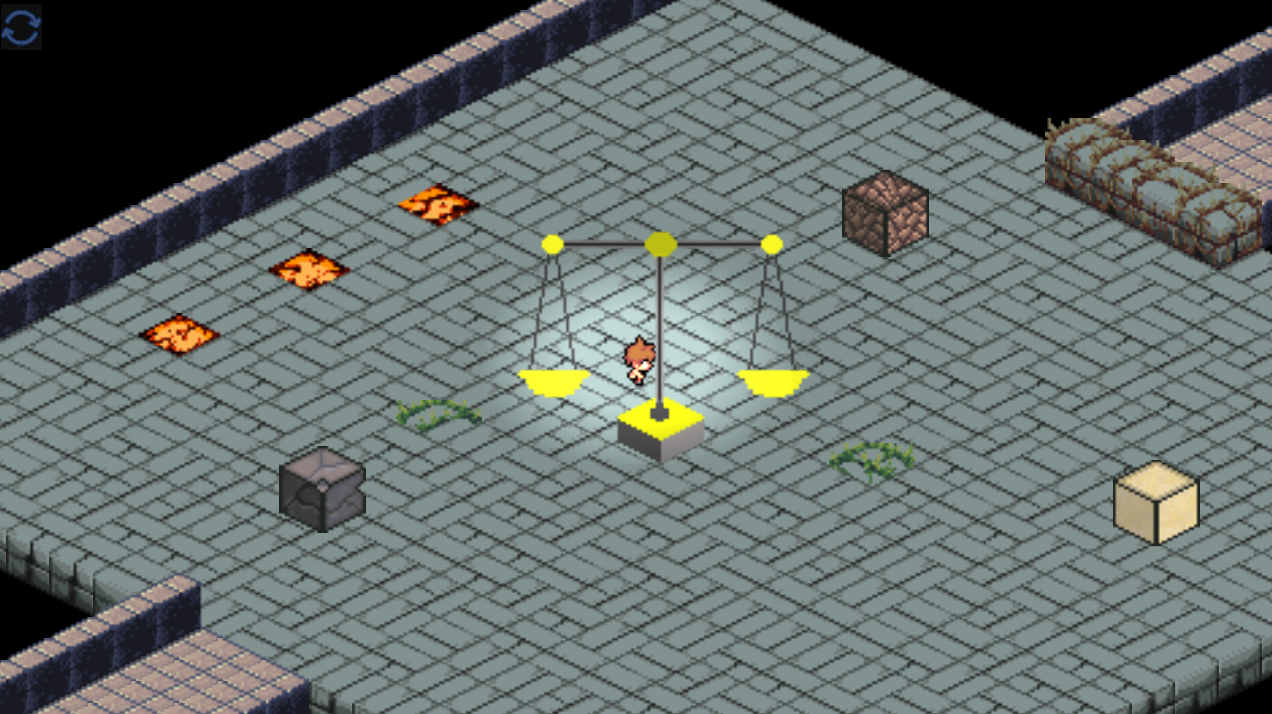
\includegraphics[width=0.7\linewidth]{Imagenes/Nivel2.png}
  \caption{Módulo mindset, imagen de referencia sobre gamificación para el módulo mindset, Nivel 2. Elaboración propia}
  \label{fig:imagen1mindset}
\end{figure}

\subsubsection{Nivel 3}
El tercer nivel se basa en un conjunto de portales: algunos permiten el paso del jugador y otros solo permiten el paso de cajas. El objetivo es llevar dos cajas hasta el final para abrir una puerta. Este nivel busca desarrollar principalmente la paciencia, ya que, al ser de varios portales, si mueves una caja demasiado rápido, podrías colocarla sobre un portal destinado solo para el jugador, lo cual te teletransportaría al tocarlo y te obligaría a reiniciar el nivel al perder acceso a la caja.

\begin{figure}[H]
  \centering
  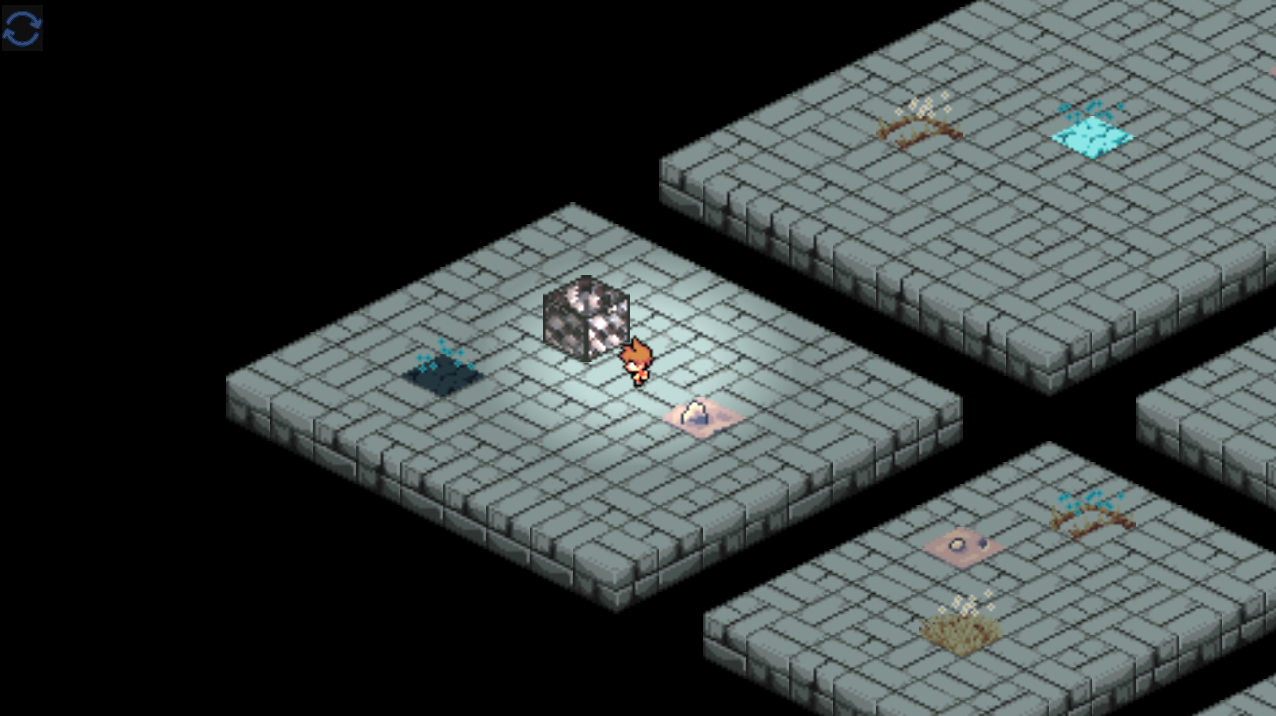
\includegraphics[width=0.7\linewidth]{Imagenes/Nivel3.png}
  \caption{Módulo mindset, imagen de referencia sobre gamificación para el módulo mindset, Nivel 3. Elaboración propia}
  \label{fig:imagen1mindset}
\end{figure}
\subsubsection{Nivel 4}
El cuarto nivel se basa en una serie de portales, donde, a partir de sutiles pistas en el escenario, el jugador puede identificar cuál es el correcto. En total, consiste en varios portales que varían en la forma de diferenciarse. Elegir un portal incorrecto devolverá al inicio del nivel, y el objetivo es fomentar la habilidad de deducción en el jugador.

\begin{figure}[H]
  \centering
  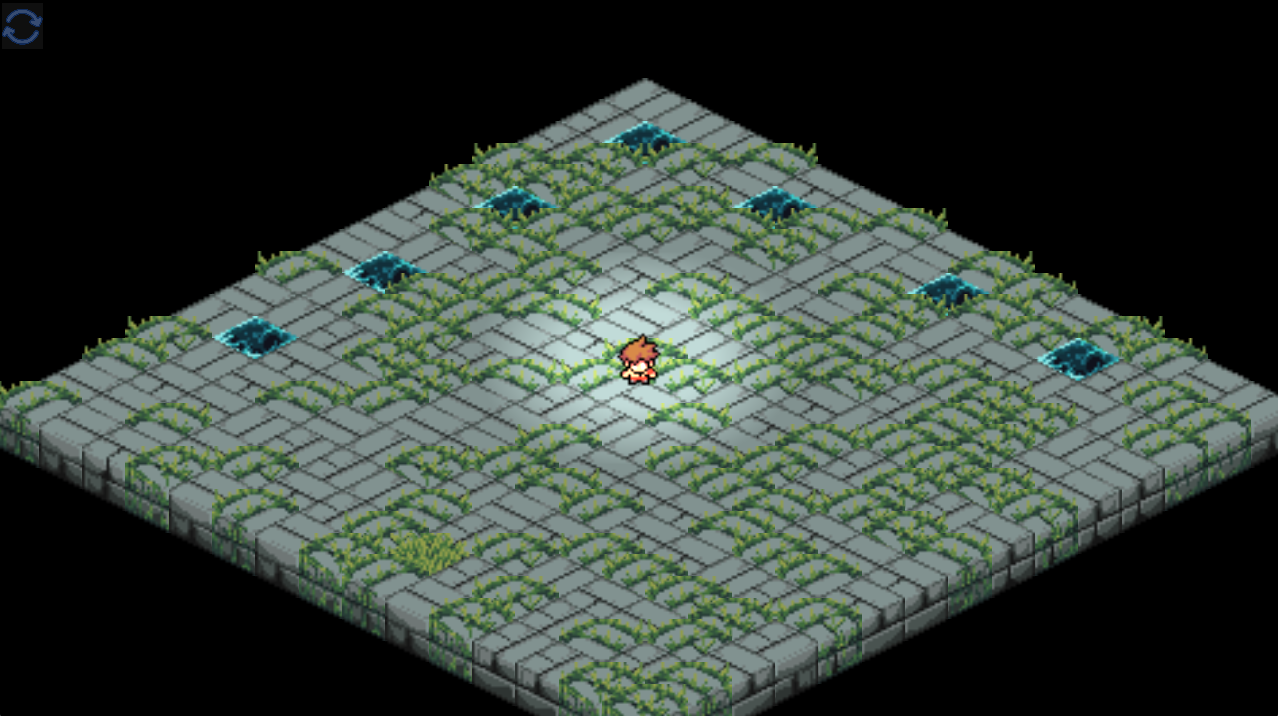
\includegraphics[width=0.7\linewidth]{Imagenes/Nivel4.png}
  \caption{Módulo mindset, imagen de referencia sobre gamificación para el módulo mindset, Nivel 4. Elaboración propia}
  \label{fig:imagen1mindset}
\end{figure}

\subsubsection{Nivel 5}
El quinto y último nivel se basa en un laberinto con visibilidad limitada, el cual tiene una sutil marca que muestra el camino correcto. Si el jugador toma un camino diferente, será devuelto al inicio del laberinto. Debido a la baja visibilidad, el jugador podría no darse cuenta de que está regresando al punto de partida, lo que puede llevarlo a dar vueltas sin saberlo. Este nivel busca fomentar tanto la capacidad de deducción como, principalmente, la paciencia del jugador, al motivarlo a probar diferentes métodos para completar el desafío.

\begin{figure}[H]
  \centering
  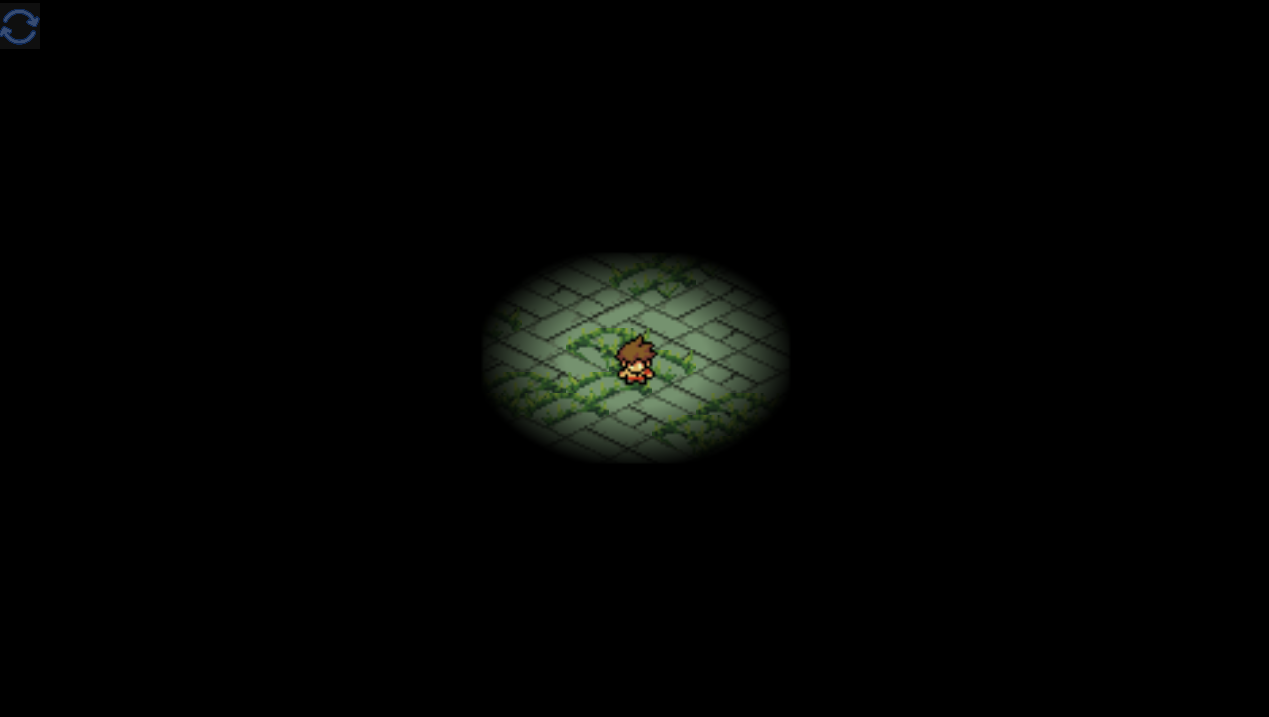
\includegraphics[width=0.7\linewidth]{Imagenes/Nivel5.png}
  \caption{Módulo mindset, imagen de referencia sobre gamificación para el módulo mindset, Nivel 5. Elaboración propia}
  \label{fig:imagen1mindset}
\end{figure}
